\documentclass[12pt]{article}
\usepackage[spanish,es-tabla]{babel}
\usepackage[utf8]{inputenc}
\usepackage[T1]{fontenc}
\usepackage{geometry}
\usepackage{setspace}
\usepackage{titlesec}
\usepackage{enumitem}
\usepackage{graphicx}
\usepackage{hyperref}
\usepackage[table,xcdraw]{xcolor}
\usepackage{tabularx}
\usepackage{colortbl}
\usepackage{ltablex}
\usepackage{tikz}
\usepackage{amsmath}
\usepackage{amssymb}
\usepackage{booktabs}
\usepackage{caption}

\setlist[itemize]{leftmargin=*,nosep,topsep=0pt,partopsep=0pt,itemsep=0.2ex,parsep=0pt}
\setlist[enumerate]{leftmargin=*,nosep,topsep=0pt,partopsep=0pt,itemsep=0.3ex,parsep=0pt}

\usetikzlibrary{shapes.geometric, arrows.meta, positioning, calc}
\keepXColumns

\geometry{a4paper, margin=2.5cm}
\setstretch{1.25}
\titleformat{\section}{\normalfont\Large\bfseries}{\thesection.}{1em}{}
\titleformat{\subsection}{\normalfont\large\bfseries}{\thesubsection.}{1em}{}

\hypersetup{
    colorlinks=true,
    linkcolor=black,
    urlcolor=blue!60!black,
    citecolor=black
}

\begin{document}

% ------------------------
% Portada
% ------------------------

\begin{titlepage}
    \centering
    \vspace*{0.5cm}
    \includegraphics[height=2.5cm,keepaspectratio]{UAEHlogo.png}\\[1.0cm]
    {\Large\bfseries PROPUESTA DE PROYECTO DE TESIS DOCTORAL \par}
    \vspace{1.0cm}
    {\large\itshape Consola Maestra Adaptativa para Cirugía Robótica \\
    basada en EEG, Inteligencia Artificial y Realidad Virtual \par}
    \vspace{8.5cm}
    {\large M.\ Eng.\ Edgar Rafael Hernández Ríos \par}
    \vspace{0.4cm}
    \begin{minipage}{0.9\textwidth}
    \centering
    Doctorado en Ciencias Computacionales \\
    Instituto de Ciencias Básicas e Ingeniería \\
    Universidad Autónoma del Estado de Hidalgo
    \end{minipage}
    \vspace{1.0cm}
    \begin{minipage}{0.9\textwidth}
    \centering
    \textbf{Director:} Dr.\ Omar Arturo Domínguez-Ramírez (UAEH) \\
    \textbf{Codirector:} Dr.\ Christian Peñaloza (Mirai Innovation Research Institute, Japón) \\
    \textbf{Asesor:} Dr.\ Carlos Trenado
    \end{minipage}
    \vfill
    {\large Pachuca de Soto, Hgo., México --- \today}
\end{titlepage}

% ------------------------
% Resumen
% ------------------------

\section{Resumen}

Esta propuesta plantea el diseño, la implementación y la validación
de una \textbf{Consola Maestra Adaptativa} para entrenamiento en
cirugía robótica, concebida como un sistema de retroalimentación
cerrada que integra electroencefalografía (EEG), inteligencia
artificial (IA) y realidad virtual (VR). El objetivo central es
ajustar dinámicamente las condiciones del entorno quirúrgico
simulado en función del estado cognitivo del usuario, estimado
mediante un índice espectral compacto basado en la razón
theta/alpha (CLI). El sistema busca mantener al aprendiz dentro
de una zona óptima de carga cognitiva durante la práctica,
optimizando así la adquisición de habilidades motoras finas y la
retención del aprendizaje.

Como base empírica, el trabajo se apoya en la validación del
índice regional
$\log\mathrm{CLI}=\overline{\log\theta_F}-\overline{\log\alpha_P}$,
computado sobre regiones frontal (F3, Fz, F4) y parietal
(P3, Pz, P4) de un sistema EEG portátil de 8 canales (AURA), en
dos paradigmas complementarios: un protocolo controlado de
lectura vs.\ Stroop y una tarea ecológica de \textit{exergaming}
interactivo (\textit{K9 CanineQuest}). Sobre esta base se define
la arquitectura de la consola adaptativa, organizada en ocho
bloques funcionales (B1--B8) y nueve lazos de comunicación (a--i)
que articulan la adquisición EEG, la detección cognitiva basada
en IA, el entorno VR adaptativo y la retroalimentación
multisensorial y háptica. El proyecto se desarrolla en
colaboración binacional entre la Universidad Autónoma del Estado
de Hidalgo y el Mirai Innovation Research Institute
(Osaka, Japón), articulando neuroergonomía, robótica y educación
médica hacia una nueva generación de simuladores quirúrgicos
inteligentes.

% ------------------------
% Introducción
% ------------------------

\section{Introducción}

La cirugía robótica es una de las áreas más avanzadas de la
medicina moderna: ofrece alta precisión, mínima invasión y mejores
resultados postoperatorios. No obstante, dominar los sistemas
quirúrgicos asistidos por robot (RAS) exige un entrenamiento
intensivo que combina habilidades motoras finas, toma de
decisiones y control cognitivo bajo alta demanda. Estudios
recientes muestran que los cirujanos, incluso expertos,
experimentan aumentos significativos en la carga mental durante
procedimientos robóticos complejos, evidenciados por la
activación de bandas theta frontales y la supresión de alpha
parietal en el EEG.

Los simuladores quirúrgicos basados en realidad virtual (VR) han
contribuido notablemente a la seguridad del aprendizaje al
permitir la práctica en entornos controlados y reproducibles. Sin
embargo, la mayoría sigue una lógica estandarizada, sin adaptarse
a las diferencias individuales en carga cognitiva, atención o
fatiga mental, limitando la eficiencia del aprendizaje. En este
contexto emergen los \textit{sistemas adaptativos}, capaces de
ajustar dinámicamente las condiciones del entorno según el estado
mental o fisiológico del usuario. Aplicar este paradigma a la
formación quirúrgica ofrece una oportunidad única para
personalizar la enseñanza, optimizar la adquisición de habilidades
y reducir la fatiga cognitiva, en concordancia con la ley de
Yerkes--Dodson.

% ------------------------
% Antecedentes
% ------------------------

\section{Antecedentes}

El EEG se ha consolidado como la herramienta más viable para
medir estados cognitivos en entornos operativos y de simulación
quirúrgica por su portabilidad, bajo costo y alta resolución
temporal. La potencia de la banda theta frontal aumenta y la
banda alpha parietal disminuye durante periodos de alta carga
cognitiva, reflejando una mayor demanda de recursos atencionales
y memoria de trabajo. En cirugía, estos patrones se correlacionan
con disminuciones en la precisión técnica y aumento de errores,
especialmente en usuarios novatos. Maimon et al.\ (2022) mostraron
que el monitoreo continuo de carga mental mediante EEG durante el
entrenamiento laparoscópico refleja la destreza adquirida: al
mejorar el desempeño, la carga cognitiva se reduce.

En paralelo, la inteligencia artificial se ha integrado en
simuladores quirúrgicos para cuantificar el rendimiento, detectar
errores y ofrecer retroalimentación personalizada. Modelos de
aprendizaje profundo permiten evaluar destreza bimanual y
predecir la tasa de aprendizaje en tareas quirúrgicas, y algunos
ensayos han demostrado que instructores virtuales basados en IA
pueden igualar o superar la eficacia de la enseñanza humana. Sin
embargo, la mayoría de estas soluciones es unidireccional: el
sistema analiza el rendimiento pero no ajusta dinámicamente el
entorno según el estado mental del aprendiz. Revisiones recientes
(Almukhtar, 2025; Wu, 2025) subrayan la ausencia de marcos
integrales de retroalimentación cerrada que combinen desempeño
técnico y estado cognitivo. Ese vacío es el que motiva este
proyecto.

% ------------------------
% Planteamiento del problema
% ------------------------

\section{Planteamiento del problema}

El entrenamiento en cirugía robótica enfrenta limitaciones tanto
pedagógicas como neurofisiológicas. La mayoría de los simuladores
actuales sigue un esquema de enseñanza estandarizado y no se
adapta al nivel de competencia ni al estado cognitivo del
aprendiz, lo que puede derivar en sobrecarga mental o baja
estimulación, afectando negativamente la retención de habilidades.
Aunque existen herramientas objetivas para medir carga mental
(EEG, fNIRS, eye-tracking), pocas plataformas las integran dentro
de un marco adaptativo cerrado; y aunque la IA se ha incorporado
en simuladores avanzados para analizar métricas de rendimiento,
no se ha implementado una integración directa entre IA y señales
neurofisiológicas que permita al sistema responder al estado
mental del aprendiz.

De este contexto surgen las preguntas guía del proyecto:
\begin{itemize}
    \item ¿Cómo integrar la medición de carga cognitiva mediante
    EEG en un simulador de cirugía robótica de forma no intrusiva
    y en tiempo real?
    \item ¿Qué variables del entorno (visual, auditiva o de
    control motor) deben modificarse para mantener al aprendiz
    dentro de una zona cognitiva óptima?
    \item ¿Es posible demostrar mejoras medibles en el aprendizaje
    quirúrgico al utilizar un sistema adaptativo neurocognitivo
    comparado con un entrenamiento estándar?
\end{itemize}

\subsection*{Pregunta de investigación}

\textit{¿Cómo diseñar e implementar una consola maestra adaptativa
que, mediante el uso combinado de EEG e IA, detecte la carga
cognitiva del usuario y modifique en tiempo real los parámetros
del entorno de realidad virtual para optimizar el aprendizaje
quirúrgico?}

% ------------------------
% Hipótesis
% ------------------------

\section{Hipótesis}

\subsection*{Hipótesis principal}

\begin{itemize}
    \item[\textbf{H1.}] \textbf{Eficacia del entrenamiento
    neuroadaptativo.} La integración de EEG, realidad virtual e
    inteligencia artificial en un bucle cerrado de
    retroalimentación mejora la eficiencia del aprendizaje en
    cirugía robótica asistida, comparada con un entrenamiento
    estándar sin adaptación cognitiva, evidenciada en mayor
    precisión técnica, menor tiempo de ejecución y mejor retención
    de habilidades motoras.
\end{itemize}

\subsection*{Hipótesis específicas}

\begin{itemize}
    \item[\textbf{H2.}] \textbf{Estabilidad del estado óptimo.} La
    condición adaptativa mantendrá al usuario dentro de una zona
    cognitiva óptima de forma más consistente que la condición no
    adaptativa, reflejada en mayor proporción de tiempo con
    $\log\mathrm{CLI}=\overline{\log\theta_F}-\overline{\log\alpha_P}$
    dentro del rango intermedio calibrado y en menor varianza
    intra-sujeto de dicho índice.
    \item[\textbf{H3.}] \textbf{Desempeño técnico y háptico.} El
    entrenamiento adaptativo se asociará con mayor precisión de
    trayectoria (menor RMSE), menor número de errores de
    manipulación, trayectorias más suaves (menor jerk medio) y
    menor fuerza pico aplicada sobre tejidos virtuales.
    \item[\textbf{H4.}] \textbf{Carga subjetiva percibida.} La
    condición adaptativa se traducirá en una carga mental
    subjetiva menor, medida con NASA--TLX global y sus subescalas
    (demanda mental, temporal, esfuerzo y frustración).
    \item[\textbf{H5.}] \textbf{Correlación dinámica
    adaptación--cognición.} Los ajustes del entorno virtual y de
    la consola háptica correlacionarán con reducciones objetivas
    de la carga cognitiva estimada por EEG en los segundos
    subsecuentes, demostrando un bucle de control funcional.
\end{itemize}

% ------------------------
% Objetivos
% ------------------------

\section{Objetivos}

\subsection*{Objetivo general}

Diseñar, implementar y evaluar una Consola Maestra Adaptativa
EEG--IA--VR que optimice el entrenamiento cognitivo y motor en
cirugía robótica, ajustando dinámicamente las condiciones del
entorno virtual según el estado mental del usuario estimado
mediante EEG y algoritmos de inteligencia artificial.

\subsection*{Objetivos específicos}

\begin{enumerate}
    \item Analizar las señales EEG relacionadas con la carga
    cognitiva y la atención sostenida durante tareas quirúrgicas
    simuladas, con énfasis en theta frontal y alpha parietal.
    \item Desarrollar algoritmos de clasificación cognitiva en
    tiempo real (SVM, redes neuronales ligeras, CatBoost) para
    estimar la carga mental del usuario a partir de
    características EEG.
    \item Diseñar estrategias de adaptación del entorno VR que
    modulen la dificultad, el ritmo y la retroalimentación
    multisensorial (visual, auditiva y háptica) según el estado
    cognitivo del usuario.
    \item Integrar los módulos EEG, IA y VR en una arquitectura
    funcional de consola maestra adaptativa, con los lazos de
    comunicación en tiempo real a--i.
    \item Validar el sistema mediante pruebas con usuarios y
    evaluar su impacto en el desempeño técnico y la carga
    cognitiva, comparando entrenamiento tradicional vs.\
    neuroadaptativo con métricas objetivas (EEG, desempeño motor)
    y subjetivas (NASA--TLX).
\end{enumerate}

% ------------------------
% Justificación
% ------------------------

\section{Justificación}

La relevancia del proyecto radica en su carácter
interdisciplinario y su potencial de innovación dentro del campo
de la cirugía robótica. Integra neurociencia, IA, VR y robótica
para desarrollar una nueva generación de simuladores quirúrgicos
adaptativos capaces de ajustar su dificultad en función del
estado cognitivo del usuario. Desde el punto de vista
\textbf{científico}, contribuye directamente al campo emergente
de la neuroergonomía quirúrgica y demuestra que los marcadores
electroencefalográficos (theta frontal, alpha parietal) pueden
utilizarse como indicadores fiables de carga cognitiva y
rendimiento técnico, transformando el EEG de una herramienta
diagnóstica pasiva en un instrumento activo de regulación del
aprendizaje.

Desde la perspectiva \textbf{tecnológica}, el proyecto propone
una arquitectura de bucle cerrado EEG--IA--VR que representa un
salto cualitativo respecto a los simuladores actuales, los cuales
sólo evalúan resultados técnicos sin considerar el estado mental
del usuario. En cuanto al \textbf{impacto educativo}, responde a
una brecha global en la formación de cirujanos: más del 70\% de
los residentes quirúrgicos en Europa y Asia no tiene acceso
regular a entrenamiento robótico, y la mayoría de los programas
carece de métricas objetivas de carga cognitiva. Finalmente, en
lo \textbf{social y contextual}, el proyecto se desarrolla como
colaboración binacional México--Japón, aprovechando la
infraestructura científica de Mirai Innovation Research Institute
y promoviendo la transferencia de tecnología, publicaciones
conjuntas y formación de recursos humanos en un área emergente.

% ------------------------
% Solución propuesta y framework
% ------------------------

\section{Solución propuesta: framework del sistema}

La propuesta consiste en una \textbf{Consola Maestra Adaptativa}
organizada como un bucle cerrado EEG--IA--VR--Usuario, estructurada
en ocho bloques funcionales (B1--B8) y nueve lazos de
comunicación (a--i). El principio de diseño es mantener al
usuario dentro de una zona óptima de carga cognitiva durante la
práctica, ajustando dinámicamente dificultad, ritmo y
retroalimentación sensorial según su estado mental estimado.

\begin{figure}[h]
\centering
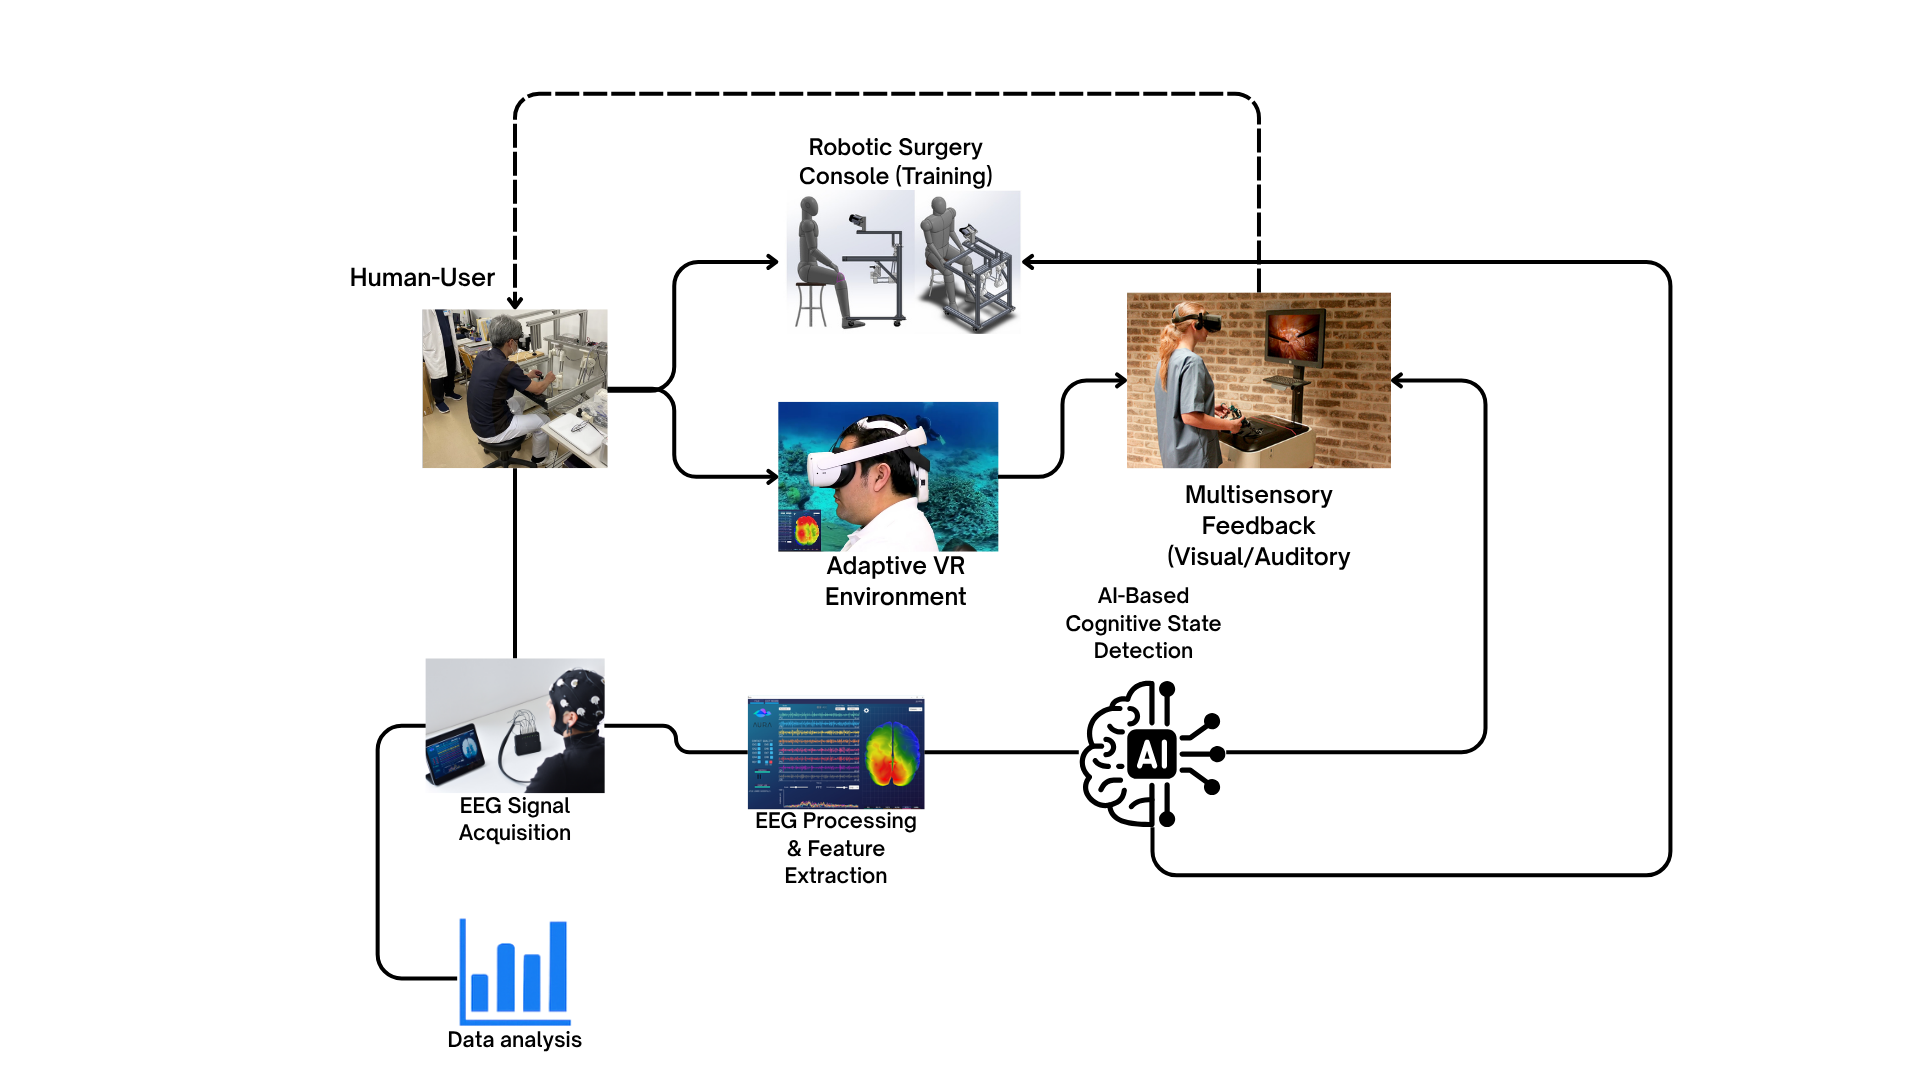
\includegraphics[width=\textwidth,keepaspectratio]{framework.png}
\caption{Framework del sistema adaptativo propuesto: bloques
funcionales (B1--B8) y lazos de señal (a--i) del ciclo cerrado
EEG--IA--VR--Usuario.}
\label{fig:framework}
\end{figure}

\subsection{Bloques funcionales}

\begin{itemize}
    \item \textbf{B1 -- Adquisición EEG.} Captura en tiempo real
    mediante un sistema EEG portátil de 8 canales (AURA)
    conectado por Lab Streaming Layer (LSL), con electrodos
    frontales (F3, Fz, F4) y parietales (P3, Pz, P4).
    \item \textbf{B2 -- Procesamiento y extracción de
    características.} Filtrado digital (1--40~Hz), eliminación de
    artefactos y cómputo de potencias espectrales en
    $\theta$~(4--7~Hz), $\alpha$~(8--13~Hz) y $\beta$~(14--30~Hz)
    por región; ventanas deslizantes de 2~s con 50\% de
    solapamiento (Welch--Hann, resolución 0.5~Hz).
    \item \textbf{B3 -- Detección cognitiva (IA).} Modelo
    supervisado interpretable (SVM, red neuronal ligera o
    CatBoost) que estima la carga (baja, óptima o alta) a partir
    del índice compacto $\log\mathrm{CLI}$ y características
    complementarias.
    \item \textbf{B4 -- Entorno VR adaptativo.} Desarrollado en
    Unity; simula tareas quirúrgicas y modifica ritmo,
    complejidad visual, auditiva o háptica según la etiqueta
    cognitiva.
    \item \textbf{B5 -- Retroalimentación multisensorial.}
    Estímulos visuales, auditivos y hápticos para apoyar la
    autorregulación cognitiva.
    \item \textbf{B6 -- Consola robótica de entrenamiento.}
    Hardware háptico (Phantom Omni/Premium, HaptX o equivalente)
    que replica la interacción física con instrumentos y modula
    resistencia, precisión y velocidad.
    \item \textbf{B7 -- Usuario humano.} Núcleo del ciclo;
    interactúa con la consola y el entorno, generando respuestas
    motoras y señales cerebrales.
    \item \textbf{B8 -- Análisis y registro.} Almacena EEG,
    etiquetas cognitivas y métricas de desempeño para análisis
    offline y refinamiento de los modelos de IA.
\end{itemize}

\subsection{Lazos de comunicación}

\begin{itemize}
    \item \textbf{a:} EEG crudo (usuario $\to$ B2). \textbf{b:}
    Características EEG ($\to$ IA). \textbf{c:} Etiqueta cognitiva
    ($\to$ VR). \textbf{d:} Parámetros adaptados ($\to$ consola).
    \item \textbf{e:} Retroalimentación de desempeño ($\to$ IA).
    \textbf{f:} Retroalimentación multisensorial ($\to$ usuario).
    \textbf{g:} Respuestas cognitivas y motoras ($\to$ EEG).
    \item \textbf{h:} Registro offline ($\to$ B8). \textbf{i:}
    Sincronización bidireccional VR $\leftrightarrow$ consola.
\end{itemize}

% ------------------------
% Metodología
% ------------------------

\section{Metodología}

El proyecto se ejecuta en cinco bloques metodológicos que se
despliegan a lo largo del cronograma (Septiembre~2025 --
Septiembre~2028):

\begin{enumerate}
    \item \textbf{Fundamentación teórica.} Revisión sistemática
    del estado del arte en neuroergonomía, cirugía robótica, EEG
    e IA aplicada; análisis comparativo de sistemas
    neuroadaptativos publicados entre 2020--2025 e identificación
    de brechas metodológicas.
    \item \textbf{Validación empírica del índice CLI.} Diseño y
    ejecución de dos paradigmas: (i) controlado
    (lectura vs.\ Stroop) y (ii) ecológico (exergaming
    \textit{K9 CanineQuest}), con pipeline de preprocesamiento
    EEG (CAR, Welch, 1--40~Hz) y análisis por modelos de efectos
    mixtos con control del efecto Berger.
    \item \textbf{Desarrollo del clasificador cognitivo.}
    Construcción del conjunto de entrenamiento con CLI y
    características espectrales complementarias; selección e
    implementación de modelos supervisados (SVM, redes neuronales
    ligeras, CatBoost); evaluación de interpretabilidad,
    histéresis y latencia EEG$\to$VR.
    \item \textbf{Construcción del sistema integrado.} Diseño e
    implementación de B1--B8 y de los lazos a--i: entorno VR
    quirúrgico en Unity, dispositivos hápticos, protocolos de
    sincronización en tiempo real, políticas de adaptación
    multisensorial y háptica, y mecanismos de calibración
    individual.
    \item \textbf{Validación experimental con usuarios.} Estudio
    comparativo intra-sujeto (24--30 participantes novatos)
    entre entrenamiento estándar y neuroadaptativo sobre la
    \emph{tarea de referencia} (sutura intracorpórea bimanual en
    VR con háptica), con análisis estadístico de efectos mixtos.
\end{enumerate}

\subsection{Tarea quirúrgica de referencia y delimitaciones}

La tarea de validación será \textbf{sutura intracorpórea
bimanual} en VR con retroalimentación háptica, seleccionada por
ser un indicador temprano de destreza en cirugía robótica, exigir
coordinación fina con incrementos robustos de theta frontal y
supresión de alpha parietal, e instrumentarse con resolución de
milisegundos. Se presentará en tres niveles de dificultad base
(bajo/medio/alto) que se ajustan cada 2--4~s según la etiqueta
cognitiva. El alcance se delimita a: usuarios novatos (estudiantes
de medicina/ingeniería biomédica en UAEH y en Japón); entorno
exclusivamente simulado (no quirófano real); EEG portátil de 8
canales; y tarea específica de sutura (no generalización a
disección, cauterización o control de cámara en este trabajo).

\subsection{Variables, métricas y KPIs}

\begin{enumerate}
    \item \textbf{Neurofisiológicas (EEG):}
    $\log\mathrm{CLI}$ regional; potencias absolutas y relativas
    en $\theta$, $\alpha$, $\beta$; \% de tiempo en zona óptima;
    varianza intra-sujeto de $\log\mathrm{CLI}$.
    \item \textbf{Desempeño técnico en VR:} tiempo de tarea,
    pasadas completadas, RMSE de trayectoria (mm), errores de
    manipulación, índice de suavidad (jerk medio).
    \item \textbf{Hápticas:} fuerza pico y media (N), simetría
    bimanual, latencia de corrección tras evento adverso (ms).
    \item \textbf{Subjetivas y conductuales:} NASA--TLX global y
    subescalas; auto-reporte de fatiga y motivación pre/post
    (Likert 1--7); eventos de adaptación disparados por el
    sistema.
\end{enumerate}

% ------------------------
% Estructura de la tesis
% ------------------------

\section{Estructura de la tesis}

La tesis se organiza en ocho capítulos que separan la
\emph{evidencia empírica} de la \emph{construcción del sistema} y
de su \emph{validación con usuarios}:

\begin{enumerate}
    \item \textbf{Cap.\ 1. Introducción.} Contexto, problema,
    hipótesis, objetivos, framework y contribuciones.
    \item \textbf{Cap.\ 2. Fundamentos y estado del arte.}
    Neuroergonomía, mecanismos theta/alpha, IA cognitiva,
    simulación VR; tabla comparativa de sistemas 2020--2025.
    \item \textbf{Cap.\ 3. Trabajo previo: validación del
    índice CLI.} Paradigmas controlado y ecológico; modelos de
    efectos mixtos; control del efecto Berger.
    \item \textbf{Cap.\ 4. Diseño e integración de la consola.}
    Arquitectura B1--B8, lazos a--i, hardware háptico, VR,
    sincronización y calibración.
    \item \textbf{Cap.\ 5. IA cognitiva en tiempo real.}
    Clasificador, interpretabilidad, histéresis, latencia
    EEG$\to$VR, integración vía LSL.
    \item \textbf{Cap.\ 6. Validación experimental.} Protocolo,
    métricas objetivas/subjetivas, análisis estadístico.
    \item \textbf{Cap.\ 7. Discusión general.} Integración de
    hallazgos, limitaciones e implicaciones.
    \item \textbf{Cap.\ 8. Conclusiones y trabajo futuro.}
    Aportaciones y líneas de extensión (fNIRS, HRV,
    pupilometría, translación clínica).
\end{enumerate}

% ------------------------
% Contribuciones propuestas
% ------------------------

\section{Contribuciones propuestas}

\begin{itemize}
    \item Marco conceptual y técnico para simulación quirúrgica
    neuroadaptativa basada en EEG.
    \item Diseño e implementación de una consola maestra
    adaptativa EEG--IA--VR, con hardware háptico y lazos de
    control en tiempo real.
    \item Modelos de IA interpretables para estimación de carga
    cognitiva y desempeño en contexto quirúrgico.
    \item Estrategias de adaptación multisensorial y háptica
    orientadas a la autorregulación cognitiva.
    \item Dataset EEG etiquetado con niveles de carga cognitiva
    durante tareas quirúrgicas simuladas.
    \item Evaluación experimental comparativa entrenamiento
    estándar vs.\ neuroadaptativo, con métricas objetivas
    (EEG, desempeño) y subjetivas (NASA--TLX).
    \item Fortalecimiento de la cooperación científica
    México--Japón en neuroeducación y robótica aplicada.
\end{itemize}

% ------------------------
% Cronograma general
% ------------------------

\section{Cronograma general (Sep.\ 2025 -- Sep.\ 2028)}

El plan de trabajo se organiza en cinco ejes: (i) investigación
y marco teórico; (ii) desarrollo experimental EEG y estimación de
carga cognitiva; (iii) desarrollo del sistema integrado
EEG--IA--RV--háptico; (iv) movilidad, difusión y publicaciones;
(v) redacción y trámites institucionales. El horizonte coincide
con el periodo de beca CONAHCyT. La residencia principal de
investigación es en Mirai Innovation Research Institute
(Osaka, Japón), con estancias periódicas en la UAEH para
revisión semestral con el comité académico.

\rowcolors{2}{gray!10}{white}
\renewcommand{\arraystretch}{1.2}

\begingroup\sloppy
\begin{tabularx}{\textwidth}{|>{\raggedright\arraybackslash}p{3.0cm}|>{\raggedright\arraybackslash}X|>{\raggedright\arraybackslash}p{3.8cm}|}
\hline
\rowcolor{gray!30}
\textbf{Periodo} & \textbf{Actividades clave} & \textbf{Entregables / Hitos} \\
\hline

\textbf{Año 1}\newline Sep.\ 2025 --\newline Jul.\ 2026 &
\begin{itemize}
  \item Revisión del estado del arte (A1).
  \item Planteamiento formal de problema, hipótesis y objetivos (A2).
  \item Diseño del protocolo EEG y selección de hardware AURA (A3).
  \item Experimentos EEG: adquisición y análisis espectral regional (A4).
  \item Clasificación ML con índice CLI y características complementarias (A5).
  \item Preparación del \textit{paper} Wiley (P1) sobre validación del CLI.
  \item Escritura continua de capítulos iniciales (T1, T2).
\end{itemize}
&
\begin{itemize}
  \item Propuesta doctoral validada.
  \item Dataset EEG inicial.
  \item Clasificador CLI piloto.
  \item Borrador \textit{paper} Wiley.
\end{itemize} \\

\hline
\textbf{Año 2}\newline Ago.\ 2026 --\newline Jul.\ 2027 &
\begin{itemize}
  \item Validación experimental del CLI con usuarios (A6).
  \item Diseño del entorno VR quirúrgico en Unity (A7).
  \item Selección y adquisición de dispositivos hápticos (A8).
  \item Estancia larga en UAEH (M2); congresos C2--C3.
  \item Envío y revisión del \textit{paper} Wiley; inicio de revisión sistemática (P2).
\end{itemize}
&
\begin{itemize}
  \item CLI validado.
  \item VR alfa + háptica integrada.
  \item \textit{Paper} Wiley publicado/en revisión.
  \item Revisión sistemática enviada.
\end{itemize} \\

\hline
\textbf{Año 3}\newline Ago.\ 2027 --\newline Jun.\ 2028 &
\begin{itemize}
  \item Integración háptica en VR con modulación por CLI (A9).
  \item Control adaptativo EEG--IA--VR--háptica en tiempo real (A10).
  \item Validación háptica con usuarios (A11).
  \item Validación del sistema completo: grupo estándar vs.\ neuroadaptativo (A12).
  \item Análisis estadístico y preparación del \textit{paper} del sistema integrado (P3).
  \item Congresos C4--C5.
\end{itemize}
&
\begin{itemize}
  \item Sistema integrado validado.
  \item Resultados comparativos.
  \item \textit{Paper} del sistema enviado.
\end{itemize} \\

\hline
\textbf{Cierre}\newline Jul.\ --\newline Sep.\ 2028 &
\begin{itemize}
  \item Revisión final por comité y autorización de impresión (T3).
  \item Trámites de titulación UAEH y cierre de beca (T4, T5).
  \item Examen recepcional y defensa doctoral.
\end{itemize}
&
\begin{itemize}
  \item Tesis impresa.
  \item Defensa doctoral (sep.\ 2028).
\end{itemize} \\

\hline
\end{tabularx}
\par\endgroup

\subsection*{Publicaciones y congresos comprometidos}

\begin{itemize}
    \item \textbf{P1.} \textit{Paper} Wiley (validación del CLI
    con experimentos EEG). Envío: ago.--dic.\ 2026.
    \item \textbf{P2.} Revisión sistemática indexada de
    neuroergonomía quirúrgica. Envío: ene.--jul.\ 2027.
    \item \textbf{P3.} Sistema integrado EEG--IA--RV--háptico
    (validación completa). Envío: ene.--jun.\ 2028.
    \item \textbf{C1--C5.} Cinco congresos internacionales
    (C1~Japón 2026; C2--C3 2027; C4--C5 2028).
\end{itemize}

% ------------------------
% Evaluación
% ------------------------

\section{Criterios de evaluación del proyecto}

\begin{itemize}
    \item \textbf{Informes semestrales y anuales} con avance
    teórico, técnico y experimental, validados por el director
    (UAEH) y el codirector (Mirai Innovation).
    \item \textbf{Validación de la propuesta doctoral} por el
    comité académico de la UAEH, incluyendo justificación
    metodológica, uso de infraestructura y plan de trabajo
    trianual.
    \item \textbf{Entrega de prototipos funcionales} del entorno
    VR, del sistema de adquisición EEG y de la consola háptica en
    cada etapa, con evidencias técnicas (bitácoras, repositorios,
    registros experimentales).
    \item \textbf{Producción académica verificable:}
    publicaciones indexadas (P1--P3), participación en congresos
    internacionales (C1--C5) y divulgación técnica.
    \item \textbf{Validación experimental con usuarios}
    demostrando mejoras estadísticamente significativas del
    entrenamiento neuroadaptativo frente al estándar en métricas
    objetivas (EEG, desempeño, hápticas) y subjetivas
    (NASA--TLX).
\end{itemize}

\end{document}
